\documentclass[11pt]{article}
\usepackage{fullpage}
\usepackage{hyperref}
\usepackage{graphicx}
\setlength{\parindent}{0cm}
%Gummi|061|=)
\title{\textbf{Beveiliging voor online bankieren}}
\author{Sander Demeester\\
		Michiel De Witte\\
		Stef Trenson}
\date{}
\begin{document}

\maketitle

\section{Inleiding}
Online bankieren en bekijken van financi\"ele informatie op een computer is onmisbaar in de digitale wereld van vandaag. Goede beveiligingsmechanismen zijn dus van cruciaal belang voor deze systemen. 

\section{Beveiligingseisen}
\label{sec:bev_eis}
\begin{itemize}
\item Privacy (tussen de gebruikers, de bank zelf moet kunnen verificeren dat het echt wel de juiste gebruiker is). De gebruiker moet kunnen vertrouwen dat de bank zijn/haar informatie geheim houd. Het limiteren van wie in de bank zelf aan welke informatie kan is hier van groot belang.
\item Vertrouwelijkheid (encryptie van gevoelige informatie)
\item Verificatie (is de informatie wel correct?)
\item Authenticatie (praat je wel met de juiste server, praat de server wel met wie hij denkt te praten?)
\item Worden betalingen en transacties correct uitgevoerd. Is er repudiation?
\item Systeem vertrouwen/persoonvertrouwen (vertrouw je iedereen die werkt in uw bank met uw gegevens). 
\item Cryptografische functies moeten veilig zijn. Maar correct gebruik in het grotere systeem is belangrijker.
\end{itemize}
We maken het onderscheid tussen 2 belangrijke zaken: 
\begin{itemize}
\item Vertrouwelijkheid van gegevens.
\item Authenticatie van entiteiten met een zo hoog mogelijke zekerheid van hun identiteit. 
\end{itemize}
\subsection{Beveiliging aanvalsvectoren}
%TODO: Hier bekijken we het threat model. Waar beschermen we tegen en vooral waar beschermen we niet tegen
We analyseren het "threat model" van ons systeem. We doen dit aan de hand van onze applicatie-eisen. We zullen mogelijke aanvalsvectoren proberen te identificeren. We herkennen dat zoiets als "perfecte beveiling" niet bestaat. Er zijn altijd meerdere partijen betrokken bij het systeem die we niet kunnen controleren en foutief gedrag van een partij kan leiden tot een gecompromitteerd systeem. Ons doel is een voldoende beveiling te garanderen voor onze resources.
\subsubsection{Authenticatie van entititen op applicatie niveau}
%TODO: bespreken wachtwoorden en andere mechanismes voor authenticatie en verificatie
%Opnemen van multifactor authenticatie en hun nut (something you are, something you know, something you have).
Waarom wachtwoorden? Wat bewijzen wachtwoorden? Waarom zijn wachtwoorden een zwakke vorm van authenticatie. Het belang van OTP en het belang van een niet-statische tweede factor. \cite{death_of_clever}\cite{pw_habit}

\subsubsection{Vertrouwelijkheid op applicatie niveau}
%TODO: bespreken van encryptie in de databank. 
Informatie die de bank over de klant opslaat in de databank is volledig ge\"encrypteerd. Een echte bank zou gebruik maken van trusted hardware encryption in het datacenter zelf. Dit was voor ons geen optie. Er gebeurd dus encryptie van de data door de database zelf (AES 256). Wachtwoord opslag doen we met bcrypt \cite{bcrypt}\ref{sec:bcrypt}. Als alternatief hier konden we scrypt, dat gebruik maakt van "memory hard problems"\cite{scrypt}. Het verschil tussen beide is dat de snelheid van bcrypt afhankelijk is van "computational speed", terwijl memory hard function vereisen dat voor elke berekening een zekere hoeveelheid fysiek geheugen moet beschikbaar zijn. En geheugen is duurder dan cpu snelheid wat resulteert in betere veiligheid.

\subsubsection{Vertrouwelijkheid op transport niveau}
%TODO: bespreken van TLS/SSL en het probleem met MITM en CBC BEAST-attack op ssl3.0/tls1.0 (opgelost in TLS1.1 maar geen goeie adoptie (gebruik van RC4 is hier een oplossing)
% bespreken van compressie probleem bij TLS (Compression Ratio Info-leak Made Easy attack)
TLS/SSL is de manier om vandaag vertrouwelijkheid te realiseren op transport/netwerk laag. We kunnen 2 groepen van problemen onderscheiden.

\begin{itemize}
\item Menselijke fouten.
\item Implementatie/algoritmische fouten.
\end{itemize}
Menselijke fouten zijn bijvoorbeeld het negeren van browser waarschuwingen en ingaan op phishing emails.
Implementatie/algoritmische fouten zijn fouten die ge\"introduceerd zijn door het beveiligingssysteem zelf (implementatie, ontwerpfouten) of door slechte configuratie van het systeem. Een voorbeeld hiervan is het gebruik van md5 voor digital signatures bij TLS/SSL (md5 second-preimage resistance is gebroken).

Om het eerste probleem op te lossen maken we gebruik van een browser feature met de naam STS (strict-transport-security). Dit is een web security policy waarbij een webserver verklaart aan web clients dat het enkel en alleen maar mag benaderd worden via een HTTPS-verbinding. HSTS heeft vele features. E\'en van deze features is dat van zodra er een fout is met het certificaat de browser zal weigeren verbinding te maken met de website. De gebruiker kan deze waarschuwing niet negeren. We merken op dat het nog steeds mogelijk is om tijdens de eerste initiele handshake het slachtoffer te worden van een MITM-aanval. Het is dan ook aangeraden om contact op te nemen met browser vendors en op de preloaded HSTS sites lijst te komen. \cite{HSTS} \cite{STS} \cite{prehsts}
\newline
Daarnaast is er een probleem bij het gebruik van CBC-encryption mode bij SSL3.0/TLS1.0. CBC mode in SSL3.0/TLS1.0 maakt gebruik van chained initialization vectors die het mogelijk maken een MITM aanval uit te voeren door een blockwise chosen-boundary aaval uit te voeren. Het resultaat is dat HTTP headers leesbaar worden en een deel vertrouwelijkheid verloren gaat.\cite{BEAST} \\

Bovendien is het mogelijk voor een hacker om session-hijacking te doen op een SSL/TLS verbinding als de verbinding compressie gebruikt. Bij deze aanval gaat niet enkel de vertrouwelijkheid verloren maar ook de authenticiteit van beide eindpunten is verloren. \cite{CRIME}\\

Verder is er ook nog een probleem met TLS/SSL renegotiation wat kan resulteren in het verliezen van vertrouwelijkheid. \cite{reg}

Het correct opzetten van een TLS/SSL webserver is niet triviaal. Ondersteuning voor oudere versies van TLS/SSL moet worden uitgezet. We opteren ook om RC4 als eerste keuze te gebruiken in onze Cipher suite.
\subsection{Mechanismen om te voldoen aan Beveiligingseisen}
Op welke manieren probeert ons syteem te voldoen aan de beveiligingseisen die worden gesteld.

\subsubsection{Multi-factor authentication}
Dit is de notie van "something you have and something you know ". 
\cite{multi_f}
Het traditioneel gebruik van wachtwoorden is niet voldoende. Wachtwoorden worden hergebruikt en zijn een single point of failure voor een authenticatie systeem. We moeten dus gebruik maken van een extra factor waar beide entititen (zowel de bank als de klant) weet van moeten hebben. Het is belangrijk dat deze factor onafhankelijk is van het systeem en niet berust op de gebruiker om iets te moeten onthouden (zoals een wachtwoord). Deze werkwijze neemt meestal de vorm aan van een hardware token. Omdat het niet mogelijk was zelf hardware tokens te maken hebben we een Android applicatie ontworpen om een deel van deze functionaliteit te simuleren.
\section{Architectuur en Implementatie}
\subsection{Architectuur}
Gekoppeld aan het gebruik van het systeem is een Android applicatie die we gebruiken voor multi-factor authenticatie in de vorm van een OTP systeem. Dit is niet ideaal omdat het geen dedicated hardware is en er de mogelijheid bestaat dat de gebruiker controle verliest over zijn smartphone.\\

De Android app maakt het ook mogelijk om aan bericht authenticatie te doen in de vorm van een HMAC die we zullen gebruiken als verificatie voor een transactie (we gaan hier later verder op in).

Tijdens het opzetten van een account zal de gebruiker persoonlijke informatie aanbieden aan de bank (via een webformulier), deze informatie bevat onder meer een door de gebruiker gekozen wachtwoord en persoonlijke informatie zoals zijn  woonplaats.\\

Voor deze informatie naar de server wordt gezonden zal op de gebruiker zijn computer het wachtwoord worden versterkt. Hiervoor maken we gebruik van een password based key derivation function \ref{sec:pbkdf2}\cite{death_of_clever} om het wachtwoord te verlengen naar 256 bits (de salt is de hash van het zelfde wachtwoord). 

We doen dit om de volgende redenen:
\begin{itemize}
\item De server kent nooit de gebruiker zijn plain text wachtwoord. 
\item De server zal deze 256 bits gebruiken om de shared key die op de server zal worden aangemaakt te encrypteren.
\end{itemize}

Deze informatie zal naar de server worden verzonden over een vertrouwlijk kanaal (ssl/tls). 
Daarna maakt de server een \emph{shared secret} aan van 512 bits met fortuna \ref{sec:fortuna}. Dit shared secret word in de database opgeslagen samen met de andere informatie en het default saldo van de gebruiker. Er is een belangrijk verschil in hoe deze informatie wordt opgeslagen. Het \emph{shared secret} wordt eerst ge\"encrypteerd met het wachtwoord dat de server ontvangt (de 256 bits output van de PBKDF2 functie). De reden hiervoor is dat de server enkel toegang mag hebben tot een plain text versie van het \emph{shared secret} als de gebruiker is ingelogd in het systeem. De andere informatie moet beschikbaar zijn, ook al is de gebruiker niet aanwezig, omdat de bank deze gegevens moet kunnen beheren.

Password storage op de server wordt gedaan door het password eerst te onderwerpen aan bcrypt \ref{sec:bcrypt}. Bcrypt is een key derivation functie die is ontworpen met 2 doelstellingen:
\begin{itemize}
\item Introduceren van een salt om rainbow tables tegen te gaan.
\item Meerdere rondes van encryptie met blowfish. Bcrypt maakt gebruik van een licht aangepaste key setup. Zowel het bericht (het wachtwoord) en de salt worden gebruikt om subkeys te maken. Het doel hiervan is om de hoeveelheid rekenkracht nodig om 1 wachtwoord te bepalen te doen stijgen. 
\end{itemize}
De reden dat we zowel hashen op de server als op de computer van de gebruiker is omdat op deze manier de server kan garanderen dat het nooit het wachtwoord van de gebruiker kent. De bank beschermt zich op deze manier tegen zichzelf \cite{pw_habit}. Daarna worden de "plain text" wachtwoorden ook nog eens veilig opgeslagen op de server met Bcrypt\cite{bcrypt}. Dit maakt het \emph{computational invisible} om de wachtwoorden te vinden met brute kracht.

Om een gebruiker uniek te identifieren wordt een unieke id aangemaakt die met de gebruiker zijn account wordt geassocieerd. Dit zal samen met het gekozen wachtwoord worden gebruikt als \'e\'en authenticatie factor van het multi-factor authenticatie proces.
	
\subsubsection{Shared secret}
Het shared secret heeft een centrale rol in ons systeem. Het wordt gebruikt om veilig in te loggen en om transacties te verif\"ieren en authenticeren. Het shared secret is een random string van 512 bits dat wordt aangemaakt met fortuna \ref{sec:fortuna}. 
Het \emph{shared secret} wordt gedeeld tussen de gebruiker en de server. We communiceren dit aan de gebruiker door het \emph{shared secret} te encoderen als een QR-code en de smartphone app deze code te laten inlezen.\\
%TODO: michiel: beschrijf hoe de app die opslaat. 
Het \emph{shared secret} wordt op 2 manieren gebruikt. \\
Tijdens het inloggen moet de gebruiker zijn ID en gekozen wachtwoord ingeven. Het wachtwoord wordt door de client terug door een PBKDF2 transformatie gestuurd en verzonden naar de server. Eerst wordt gecontroleerd of het wachtwoord correct is door Bcrypt te gebruiken en te vergelijken met het resulaat in de databank. Als de verificatie slaagt zal het origineel verzonden wachtwoord (de output van de PBKDF2 functie op de client) worden gebruikt om het \emph{shared secret} te decrypteren in de databank. Voor de rest van de sessie zal een  plain text versie van het \emph{shared secret} beschikbaar zijn op de server.

Op dit moment beschikken zowel de server als de gebruiker over het shared secret. De server voert een \emph{challenge and response} protocol uit om te controleren of de gebruiker beschikt over het correcte \emph{shared secret}.\\

\subsubsection{Challenge and response}
De manier waarop de server dit doet is de volgende, de server genereert 8 random bytes gebruik makende van fortuna \ref{sec:fortuna}. Deze 8 random bytes worden in de vorm van een QR-code aan de client gepresenteerd. De client gebruikt de smartphone app om deze 8 random bytes te verwerken op de volgende manier.\\

We nemen de unix time en introduceren een tijdsraam van 30 seconden. Daarna xor'en we de 8 random bytes met de unix time.

We merken op dat enkel de response een geldigheidsduur bevat in de response zelf. Dit is niet het geval voor de challenge. De reden is dat de response een waarde heeft in het systeem, het is nl. de tweede factor. Een bovengrens voor de tijd op de server is natuurlijk de tijd tot de http sessie verloopt.

Daarna gebruiken we een Time-Based One-Time Password Algorithm \ref{sec:totp} met als key het \emph{shared secret} en als tijd factor de 8 bytes ge-xored met de unix time. We herkennen het probleem dat ongeveer de 32 minst significante bits zullen worden be\"invloed door de tijd. Dit is niet echt een probleem omdat de overige bits ook random zijn.

De gebruiker voert het Time-Based One-Time Password algoritme uit met als key het \emph{shared secret} en als message de 8 bytes. Het resultaat is een token van 8 digits lang die afhankelijk is van de server zijn \emph{challenge}, een tijdsfactor en het \emph{shared secret}. De gebruiker stuurt dit terug naar de server. De server beschikt over de zelfde informatie op de exacte tijd na, maar is in staat om het tijdsvenster van de response te controleren. We erkennen het probleem dat de tijd op de server en client kan verschillen. De server zal hier dan ook rekening mee houden.\\

De tweede manier waarop het \emph{shared secret} wordt gebruikt is tijdens het authenticeren en het verif\"ieren van een transactie.

\subsubsection{Verificatie en authenticatie van een transactie}
Op het moment dat de gebruiker een transactie wil uitvoeren zal de server een hash-based message authenticatie code bepalen van de transactie (HMAC). Op dit moment is de gebruiker ingelogd en heeft het systeem toegang tot de plain text versie van het \emph{shared secret}. Dit \emph{shared secret} zal als key worden gebruikt (herinner dat het \emph{shared secret} 512 bits lang is). Als key voor het HMAC bericht wordt alle informatie in de transactie samen beschouwd (inclusief de tijd op het moment van de transactie zelf). \\

Het is enkel mogelijk om een geldige HMAC te bepalen van een transactie als de gebruiker is ingelogd en zijn \emph{shared secret} is gedecrypteerd.\\

Deze HMAC kan later worden gebruikt als verificatie van de transactie, nl: "Het is enkel mogelijk dat deze HMAC is gemaakt met een plain text versie van het \emph{shared secret}". Dit impliceert dat de maker van de HMAC kennis moet hebben van het \emph{shared secret} in plain text, de bank heeft hiertoe enkel toegang als de gebruiker is ingelogd in het systeem.\\


We gebruiken hier een HMAC in tegenstelling tot een gewone bericht authenticate om de length extension attack te voorkomen.\\

Eenmaal de HMAC is berekend nemen we de 64 minst significante bits en maken terug een QR-code en voeren we opnieuw het bovenstaande challenge en reponse protocol uit. Dit resulteert in transactie authenticatie. Dit bewijst enkel dat op het huidige moment een persoon met kennis van het \emph{shared secret} en de challenge (de 64 minst significante bits) deze transactie goedkeurt. Het systeem zal enkel een transactie uitvoeren als de response code geldig is. Dit slaan we ook op in de databank samen met de HMAC.
\subsubsection{Account security assets}
Inloggen bestaat uit 2 fases: het aanbieden van het ID en wachtwoord en het uitvoeren van de challenge en response procedure. Het systeem zal pas een melding geven dat de login foutief was nadat de gebruiker een response code heeft ingegeven, ook al is de combinatie van ID en wachtwoord foutief. Dit is om geen informatie te lekken of duidelijk te maken welk deel van de login procedure foutief is.\\

Bij drie foute login pogingen moet de gebruiker contact met de bank opnemen om zijn account te resetten. Dit houdt in dat een nieuwe \emph{shared secret} zal moeten worden aangemaakt.
\subsection{Implementatie}
\subsubsection{Android APP}
De android app bevat ook het shared secert. Het is dus hier ook van groot belang dat dit veilig gebeurd. 
De android app is beschermd met een 4 digit PIN. Het shared secret zelf is met AES geencrypteerd. 

We herkennen het probleem dat, in tegenstelling tot andere banken we niet kunnen gebruik maken van speciale hardware tokens. Als de gebruiker controle verliest over zijn smartphone is het triviaal op de geencrypteerde shared secert op te zoeken in de app en deze met brute kracht de PIN proberen te achterhalen. 

Als dit zou gebeuren dat bezit de aanvaller enkel en alleen 
\subsubsection{Random events}
Random data is belangrijk. De 8 bytes login tokens en het \emph{shared secret} maken er gebruik van.
De initi\"ele seed voor fortuna hangt dan ook af van externe factoren. We gebruiken hiervoor de system timer. Het verschil tussen 2 oproepen is meestal in de orde van $2^63$, maar aangezien het return type 64 bit is zal er dus vaak numurieke overflow zijn. Daarnaast gebruiken we nog het aantal beschikbare CPU's en fysiek geheugen dat beschikbaar is tijdens het opstarten van de applicatie.
\subsubsection{Fortuna}
\label{sec:fortuna}
De reden waarom we hebben gekozen voor fortuna als PRNG is voor de entropy accumulator. Fortuna maakt gebruik van entropy pools. Elke entropy source verdeelt informatie over deze pools wanneer de PRNG opnieuw word geseed. In het geval van onze applicatie is dat voor het aanmaken van nieuwe random bytes.

\subsubsection{Time-based One-time Password Algorithm}
\label{sec:totp}
We maken gebruik van het TOTP protocol beschreven in RFC 6238.
$$ TOTP = Truncate(HMAC-SHA512(K,M))$$
Waar $K$ het \emph{shared secret} is en $M$ de \emph{message} is die bestaat uit 8 bytes. Als de server een response code ontvangt controleert deze dat ze ofwel in het huidige tijdsvenster valt of in het tijdsvenster ervoor. We herkennen het probleem dat een tijdscode kan worden gemaakt naar het einde toe van het huidige tijdsvenster, zodat als de server de code verwerkt er al een nieuw tijdsvenster kan aangebroken zijn.\\

TOTP maakt gebruikt van een HMAC. We gebruiken hier sha256 als onderliggend hashing algoritme omdat deze een blok lengte heeft van 512 bits. Dit is evenveel als het \emph{shared secret} (dit geldt ook voor de transactie)
\subsubsection{PBKDF2}
\label{sec:pbkdf2}
Omdat het wachtwoord van de gebruiker zal worden gebruikt als sleutel $S_{0}$ voor het encrypteren van het \emph{shared secret} op de server is het belangrijk dat deze sleutel de correcte lengte heeft en dat deze moeilijk te achterhalen zou zijn met brute kracht. De output van de PBKDF2 functie ($S_{0}$) is 256 bits die in zijn volledigheid naar de server wordt verstuurd.\\

Het is hierbij van groot belang dat voor de server probeert het \emph{shared secret} te decrypteren met $S_{0}$ het eerst verifieert dat $S_{0}$ correct is door Bcrypt te gebruiken en te vergelijken met de waarde in de databank. Als dit niet gebeurt kan de integriteit van het systeem niet worden gegarandeerd. 
\subsubsection{Bericht authenticatie}
\label{sec:mac}
Het is moeilijk om traditionele digitale handtekeningen te gebruiken omdat we moeten vertrouwen op informatie die de gebruiker intypt. Als alternatief maken we gebruik van authenticatie codes met een shared secret. Het probleem met hashes van de vorm $H(key || message)$ is dat deze kwetsbaar zijn voor een Length extension attack als gevolg van de Merkle–Damgard construction\cite{len_ext_attack}. Omwille van deze reden gebruiken we een HMAC voor bericht authentitcatie.
\subsubsection{Account beveiliging}
\label{sec:bev}
Standaard beleid voor account reset en wachtwoord verlies. De gebruiker kan contact opnemen met de bank om zijn account te laten blokkeren of een nieuw \emph{shared secret} aan te vragen. Ook als de gebruiker 3 keer foutief inlogt zal zijn account worden geblokkeerd en moet er contact worden opgenomen met de bank.\\

Het systeem houdt ook bij wie al is ingelogd, zodat een tweede login poging voor een sessie die bezig is zal worden gezien als een aanvalspoging.
\section{Problemen}
\subsection{Algemene problemen en hun oplossingen}
De denkwijze die we tijdens dit project hanteerden is die van "Professional Paranoia". We gaan er ook vanuit dat de gebruiker zijn computer gecompromitteerd is en de aanvaller alles kan zien.

\subsubsection{Inlog procedure}
Het is enkel mogelijk om in te loggen als de persoon beschikt over de correcte ID en het gekozen wachtwoord. Het is niet mogelijk om de ssl/tls verbindingen af te luisteren wegens het gebruik van STS (strict-transport-security). Zowel de gebruiker als de bank beschikken over het ID, maar enkel de gebruiker beschikt over het gekozen wachtwoord (de bank heeft enkel een ge\"encrypteerde versie van het wachtwoord en krijgt nooit de plain-text versie te zien). Dit is de "something you know"-factor.

Daarnaast hebben we ook nog de "something you have"-factor, met name het \emph{shared secret}. Enkel de gebruiker beschikt over deze informatie in de Android app. We herkennen het probleem dat de gebruiker deze informatie kan verliezen. Maar de app beschikt enkel over het \emph{shared secret}, niet over de gebruiker zijn ID of wachtwoord.\\

Er kan eventueel het probleem zijn dat de gebruiker zijn machine gecompromitteerd is. Dit wil zeggen dat het ID en wachtwoord gekend zijn. Het is voor een aanvaler niet mogelijk om informatie over het \emph{shared secret} te halen uit de response van de gebruiker. Ook kan deze response niet worden herbruikt want zodra de response gemaakt wordt krijgt ze een waarde in het protocol en de versheid wordt beschermd door de tijd.

\subsubsection{Authenticatie en verificatie van transacties}
We beschouwen twee delen in dit proces:
\begin{itemize}
\item Verificatie in de huidige tijd en op latere tijdstippen.
\item Authenticatie in de huidige tijd.
\end{itemize}
Verificatie in de huidige tijd gebeurt door een combinatie van 2 dingen: de gebruiker is ingelogd en de server heeft toegang tot het \emph{shared secret} \'en de gebruiker kan bewijzen dat hij toegang heeft tot het zelfde \emph{shared secret} door terug de \emph{challenge response} procedure te doorlopen met de 64 minst significante bits van de HMAC. Als de server de response niet kan verif\"ieren kan de transactie niet doorgaan. Deze 2 eisen zijn voldoende voor authenticatie en verificatie in de huidige tijd. \\

Verificatie van een transactie op een later tijdstip kan worden gedaan als de gebruiker het \emph{shared secret} op de server decrypteert. Enkel de gebruiker kon deze transactie doen want enkel hij beschikt over het wachtwoord om de bank toegang te geven zijn \emph{shared secret}. Daarnaast moeten alle stappen van het systeem worden uitgevoerd alvorens het mogelijk is een transactie uit te voeren. Dus moet authenticatie ooit hebben plaats gevonden.
\section{Conclusie en observaties}
"Information security is hard". Er zijn altijd factoren in het spel waarmee we geen rekening kunnen houden. En om te zeggen dat onze beveiling perfect is, of te zeggen dat ze goed is zou onze eerste grote fout zijn. Wat we kunnen doen is hopen. Hopen dat onze beveiliging "goed genoeg" is. We moeten steeds veronderstellen dat er fouten zijn, die noch door ons noch door de aanvallers gevonden zullen worden.
\begin{center}
\begin{figure}
\fbox{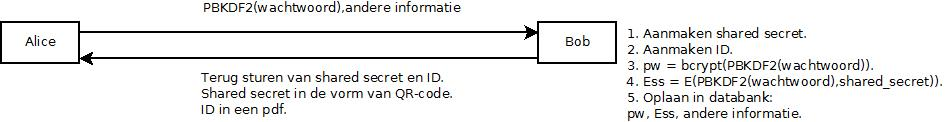
\includegraphics[width=180mm]{registreren.jpg}}
\caption*{Registeren diagram}\label{fig:registeren}
\end{figure}
\begin{figure}
\fbox{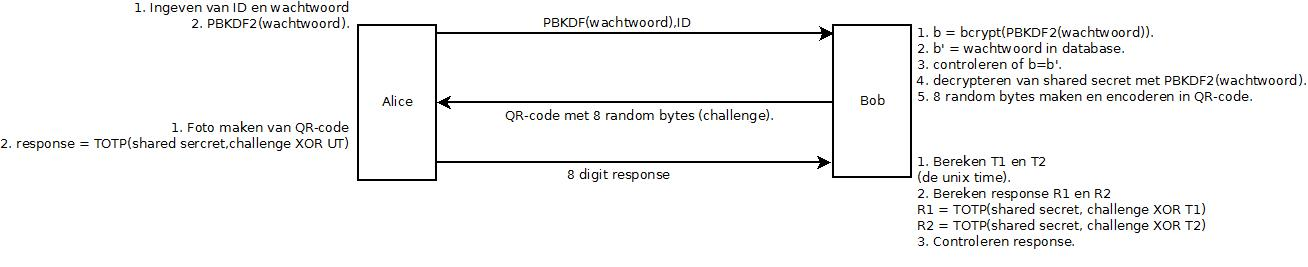
\includegraphics[width=180mm]{inloggen.jpg}}
\caption*{Inloggen diagram}\label{fig:inloggen}
\end{figure}
\begin{figure}
\fbox{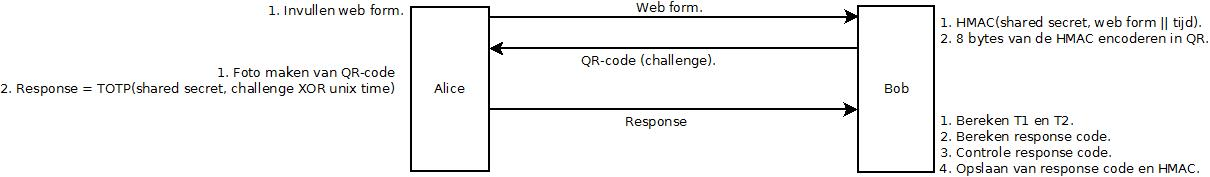
\includegraphics[width=180mm]{transactie.jpg}}
\caption*{Transactie uitvoeren}\label{fig:transactie}
\end{figure}
\end{center}
\newpage
\begin{thebibliography}{9}
\bibitem{CRIME}
  John Kelsey,
  \emph{{{C}ompression and {I}nformation {L}eakage of {P}laintext}}.
  Fast Software Encryption, 9th International Workshop,
  2nd Edition,
  2002.
\bibitem{BEAST}
	Juliano Rizzo en Thai Duong,
	\emph{Browser Exploit Against SSL/TLS}. De "BEAST"-attack.
\bibitem{reg}
	\emph{Protect your server against TLS renegotiation and man-in-the-middle vulnerabilities.}
	\url{https://www.digicert.com/news/2011-06-03-ssl-renego.htm}

\bibitem{TOTP}
	 D. M'Raihi,  S. Machani, M. Pei en  J. Rydell,
	 \emph{TOTP: Time-Based One-Time Password Algorithm}
	 RFC 6238,
\bibitem{len_ext_attack}
	G. Tsudik,
	\emph{Message authentication with one-way hash functions} en
	\emph{http://www.vnsecurity.net/t/length-extension-attack/}
	
\bibitem{fortuna}
	Bruce Schneier en Niels Ferguson
	\emph{Fortun PRNG}
\bibitem{AP}
	Bruce Schneier
	\emph{Applied cryptography}
\bibitem{CE}
	Niels Ferguson, Bruce Schneier, and Tadayoshi Kohno,
	\emph{Cryptography Engineering: Design Principles and Practical Applications}
\bibitem{bcrypt}
	Niels Provos en David Mazieres,
	\emph{Future-Adaptable Password Scheme - OpenBSD}
\bibitem{scrypt}
	Colin Percival,
	\emph{Stronger Key Derivation via Sequential Memory-hard functions}
	\url{www.tarsnap.com/scrypt/scrypt.pdf}
\bibitem{multi_f}
	Jon Oberheide,
	\emph{Multi-factor authentication Past, Present and future}.\\
	CTO, Scio Security
\bibitem{pbkdf2}
	Meltem sonmez turan, Elainse barker, Wiliam burr en Lily chen,
	\emph{Recommandations for password-based key derivation}\\
	\url{http://csrc.nist.gov/publications/nistpubs/800-132/nist-sp800-132.pdf}
\bibitem{death_of_clever}
	Bill Ricker,
	\emph{Passwords "The death of clever"}, 
	BLU.org 2012-09-19. \\
	\url{blu.org/meetings/2012/09/Passwords.pdf‎}
\bibitem{forward_secret}
	Gene Itkis,
	\emph{Forward security: Adaptive Cryptograpy: Time evolution}
	Computer Sience Department, Boston University.\\
	\url{http://www.cs.bu.edu/~itkis/pap/forward-secure-survey.pdf}
	
\bibitem{pw_habit}
	Dinei Florencio en Cormac Herley,
	\emph{A Large-Scale Study of Web Password Habits}
	Microsoft Research.\\
	\url{https://research.microsoft.com/pubs/74164/www2007.pdf}
\bibitem{HSTS}
  The Chromium Project
  \emph{HTTP Strict Transport Security}
  \url{http://www.chromium.org/sts}
\bibitem{STS}
  J. Hodges, C. Jackson en A. Barth
  \emph{RFC Strict-Transport-Security}
  \url{https://tools.ietf.org/html/rfc6797}
\bibitem{prehsts}
  Mozilla Security Blog
  \emph{Preloading HSTS}
  \url{https://blog.mozilla.org/security/2012/11/01/preloading-hsts/}
\end{thebibliography}
\end{document}
